\documentclass[11pt]{article}
\usepackage[top=56pt,bottom=58pt,left=50pt,right=48pt]{geometry}
%\usepackage{apacite}

\usepackage[
backend=biber,
style=nature,
]{biblatex}
\title{A bibLaTeX example}
\addbibresource{citations.bib} %Imports bibliography file


\usepackage[slovene]{babel}
\usepackage{amsmath}
\usepackage{color}
%\usepackage{graphicx,subfigure}

%\usepackage{subfigure}

\usepackage[T1]{fontenc}
\usepackage[utf8]{inputenc}
\usepackage{lmodern}
\usepackage{amsmath}
\usepackage{tikz}
\usetikzlibrary{shapes,shapes.geometric,arrows,fit,calc,positioning,automata}

\usepackage{amsfonts}
\usepackage{mathrsfs}

\usepackage{float}

\usepackage{caption}
\usepackage{subcaption}

\usepackage{enumerate}
\usepackage{slashed}

%\usepackage{natbib}

%\usepackage{chemformula}
%\usepackage[version=4]{mhchem}
%\usepackage{mychemistry}
%\usepackage{chemfig}

%\def\phi{\varphi}
%\def\eps{\varepsilon}
%\def\theta{\vartheta}

%\usepackage{physics} ta je za vektorje: \vectorbold{}

\newcommand{\thisyear}{2020/21}

\renewcommand{\Re}{\mathop{\rm Re}\nolimits}
\renewcommand{\Im}{\mathop{\rm Im}\nolimits}
\newcommand{\Tr}{\mathop{\rm Tr}\nolimits}
\newcommand{\diag}{\mathop{\rm diag}\nolimits}
\newcommand{\dd}{\,\mathrm{d}}
\newcommand{\ddd}{\mathrm{d}}
\newcommand{\ii}{\mathrm{i}}
\newcommand{\lag}{\mathcal{L}\!}
\newcommand{\ham}{\mathcal{H}\!}
\newcommand{\four}[1]{\mathcal{F}\!\left(#1\right)}
\newcommand{\bigO}[1]{\mathcal{O}\!\left(#1\right)}
\newcommand{\sh}{\mathop{\rm sinh}\nolimits}
\newcommand{\ch}{\mathop{\rm cosh}\nolimits}
\renewcommand{\th}{\mathop{\rm tanh}\nolimits}
\newcommand{\erf}{\mathop{\rm erf}\nolimits}
\newcommand{\erfc}{\mathop{\rm erfc}\nolimits}
\newcommand{\sinc}{\mathop{\rm sinc}\nolimits}
\newcommand{\rect}{\mathop{\rm rect}\nolimits}
\newcommand{\ee}[1]{\cdot 10^{#1}}
\newcommand{\inv}[1]{\left(#1\right)^{-1}}
\newcommand{\invf}[1]{\frac{1}{#1}}
\newcommand{\sqr}[1]{\left(#1\right)^2}
\newcommand{\half}{\frac{1}{2}}
\newcommand{\thalf}{\tfrac{1}{2}}
\newcommand{\pd}{\partial}
\newcommand{\Dd}[3][{}]{\frac{\ddd^{#1} #2}{\ddd #3^{#1}}}
%\newcommand{\Pd}[3][{}]{\frac{\pd^{#1} #2}{\pd #3^{#1}}}
\newcommand{\avg}[1]{\left\langle#1\right\rangle}
\newcommand{\norm}[1]{\left\Vert #1 \right\Vert}
\newcommand{\braket}[2]{\left\langle #1 \vert#2 \right\rangle}
%\newcommand{\obraket}[3]{\left\langle #1 \vert #2 \vert #3 \right \rangle}
%\newcommand{\hex}[1]{\texttt{0x#1}}
\newcommand{\vect}[1]{\boldsymbol{#1}}

\renewcommand{\iint}{\mathop{\int\mkern-13mu\int}}
\renewcommand{\iiint}{\mathop{\int\mkern-13mu\int\mkern-13mu\int}}
\newcommand{\oiint}{\mathop{{\int\mkern-15mu\int}\mkern-21mu\raisebox{0.3ex}{$\bigcirc$}}}

\newcommand{\wunderbrace}[2]{\vphantom{#1}\smash{\underbrace{#1}_{#2}}}

\renewcommand{\vec}[1]{\overset{\smash{\hbox{\raise -0.42ex\hbox{$\scriptscriptstyle\rightharpoonup$}}}}{#1}}
\newcommand{\bec}[1]{\mathbf{#1}}
\newcommand{\q}[1]{``#1''}
\newcommand{\s}[1]{\s{#1}}
\newcommand{\tr}{\mathbf{Tr}}

\newcounter{daggerfootnote}
\newcommand*{\daggerfootnote}[1]{%
    \setcounter{daggerfootnote}{\value{footnote}}%
    \renewcommand*{\thefootnote}{\fnsymbol{footnote}}%
    \footnote[2]{#1}%
    \setcounter{footnote}{\value{daggerfootnote}}%
    \renewcommand*{\thefootnote}{\arabic{footnote}}%
    }



\begin{document}


\begin{titlepage}
\begin{center}
	
	{\sc\Large	Teorija osnovnih delcev in jedra}\\
	\vspace*{5cm}
	\LARGE\textbf{Anihilacija $e^+ e^-$ v tri hadronske curke}\\
	\vspace{0.2cm}
	\vspace{1.6cm}
	\large{Avtor: Žan Butala}\\
	\text{vpisna številka: 28222060}
 
      % \vspace{1cm}
	%\begin{figure}[H]
   %	 \centering
    %	\includegraphics[width=10cm]{semafor1.png}
    	%\label{fig:graf1}
	%\end{figure}

       \vspace{5cm}


       \vfill

	\normalsize
 
       {\sc 28. april 2024\\
	\vspace{0.2cm}
       Univesity of Ljubljana\\
       Faculty of mathematics and physics\\}
      
\end{center}
\end{titlepage}


\newpage

\tableofcontents







\vspace*{0.5cm}
\section{Uvod}

V nalogi se lotimo anihilacije elektrona in pozitrona v tri hadronske curke.
Anihilacija e+ e-, v nasprotju s trki hadronov, zagotovi čisto reakcijo (brez množice vmesnih stanj).
Virtualni foton, ki pri tem nastane, lahko razpade v pare lepton-antilepton ali v par kvark-antikvark
(v tej nalogi ne upoštevamo šibke interakcije, kjer nastane $Z^0$).
Osredotočimo se na slednji primer v limiti visokih energij, kjer je sklopitev $\alpha_s$ majhna in lahko uporabimo perturbativni pristop.
Procesu ustreza Feynmannov diagramom \ref*{fig:expb}, 
ki mu bomo kasneje dodali še izsev gluona iz enega izmed kvarkov \ref*{fig:expc}.
Iskaže se, da ta proces vodi do tvorbe treh hadronskih curkov.

Ujetost barv narekuje, da so v QCD asimptotska stanja barvni signleti SU(3).
S cepitvijo barvnega singleta na njegove komponente, npr. mezon v kvark in antikvark, pridelamo vmesno privlačno polje s konstantno energijsko gostoto,
s čimer je energija, ki jo nosi, sorazmerna z razdaljo.
Posledično v eksperimentih ne opazimo prostih kvarkov, temveč hadronske curke.
Nastanek hadronskega curka iz kvarka je neperturbativen proces, vendar v limiti kratkih razdalj lahko vseeno
uporabljamo perturbativen pristop in Feynmannove diagrame, ker asimptotska svoboda poskrbi za šibko efektivno sklopitev in

Eksperimentalne meritve podajajo skalo močne interakcije, z vrednostjo $\Lambda \sim 220 \, \mathrm{MeV}$.
Perturbacijska QCD je torej veljavna pod skalo $\sim 1/\Lambda \approx 1 \, \mathrm{fm}$,
kar je približno razsežnost lahkih hadronov \cite*{peskin}.






\vspace*{0.5cm}
\section{Anihilacija $e^+e^-$ v $q\bar{q}$}
Spomnimo se na soroden proces, ki smo ga obravnavali že pri JKL, to je sipanje $e^+e^-$ v $\mu+\mu-$.
Sipalni presek za ta proces je:
\begin{equation}
       \sigma_0 \equiv \sigma (e^+e^- \rightarrow \mu^+ \mu^-) = \frac{4 \pi \alpha^2}{3 Q^2}.
\end{equation}
Skoraj identičen izraz dobimo, če končno stanje zamenjamo s parom kvark-antikvark:
\begin{equation}
       \sigma (e^+e^- \rightarrow q \bar{q}) = 3 e_q^2 \sigma_0,
\end{equation}
kjer smo upoštevali neceli naboj kvarka $E$, faktor 3 pa je posledica barvnih kanalov.
Od tod lahko napovemo sipalni presek, kjer so končno stanje hadroni:
\begin{equation}
       \sigma (e^+e^- \rightarrow \text{hadroni}) = \sum_q 3 e_q^2 \sigma_0,
       \label{eq:gornji}
\end{equation}
kjer vsota teče po vseh kvarkovskih okusih.
Zgornja obravnava je zgolj reda $\mathcal{O}(\alpha^2)$.
Naslednji red, ki ga lahko vključimo v obravnavo je $\mathcal{O}(\alpha^2 \alpha_s)$.

%Pri upoštevanju popravka h kvarkovskem verteksu se izkaže, da se divergentni členi ravno
%pokrajšajo, gornji rezultat pa se modificira v obliko:
%\begin{equation}
%       \sigma (e^+e^- \rightarrow \text{hadroni}) = \sum_q 3 E^2 \sigma_0 \Big (1 + \frac{\alpha_s(Q^2)}{\pi} \Big),
%\end{equation}

%V drugem redu $\mathcal{O}(\alpha^2)$ dobimo dva hadronska curka, $\alpha^2 \alpha_s$ pa tri.
%V slednjem primeru ima tretji curek gluon za starševki parton.
%Pri visokih energijah $Q^2$, kjer je $\alpha_s(Q^2) \approx 0.1$, dobimo tri hadronske curke v 10\% dogodkov.













\section{Tri hadronski curki}
V nalogi bomo obravnavali stanja v limiti visokih energij, torej lahko njihove mase zanemarimo.
Dodatno bomo posplošili obravnavo gluona, ki mu bomo pripisali majhno maso $\mu$, da se bomo lahko izognili logaritemskim divergencam pri vmesnih rezultatih.
Nakoncu jo bomo poslali proti nič.



\subsection{Fazni integral po končnih stanjih}
Definirajmo najprej kinematične spremenljivke.
Vpadna elektron in pozitron naj imata četverca gibalne količine $k_{e-}$ in $k_{e+}$.
Četverec virtualnega fotona, ki nastane pri anihilaciji e+e-, označimo s $q$.
Četverca nastalega kvarka in antikvarka označimo s $p_q$ in $p_{\bar{q}}$ ter izsevanemu gluonu pripišemo $p_g$.
%Od Mandelstamovih spremenljivk, če prav bomo zares rabili le $s$:
%\begin{equation}
%       \begin{split}
%              s &= (k_{e-} + k_{e_+})^2, \\
%              t &= (k_{e-} - (p_q + p_g) )^2, \\
%              t &= (k_{e-} - p_{\bar{q}} )^2.
%       \end{split}
%\end{equation}
Prikladno je uvesti nov set brezdimenzijskih spremenljivk
\begin{equation}
       x_i = \frac{2 p_i \cdot q}{q^2},
\end{equation}
kjer $i$ teče po končnih stanjih.
V težiščnem sistemu potem direktno velja $x_i = 2E_i/q^0$, kar so ravno pripadajoči deleži energije, ki je na voljo.
Uporabno je pokazati tudi, kako se Lorentzovi skalarji izražajo z mirovno maso in deležem energije $x_i$:
\begin{equation}
       \begin{split}
              (p_q + p_{\bar{q}})^2 =& (q - p_g)^2 = q^2 - 2 q \cdot p_g + p_g^2 = s (1-x_3) + m_3^2, \\
              (p_{\bar{q}} + p_g)^2 =& s(1-x_1) + m_1^2, \\
              (p_g + p_q)^2 =& s(1-x_2) + m_2^2
       \end{split}
       \label{eq:pokazi}
\end{equation}
%ter da je vsota
%\begin{equation}
%       \sum_i x_i = 2.
%\end{equation}

V naslednjem koraku poenostavimo fazni integral za tri delce v končnem stanju težiščnega sistema
\begin{equation}
       \int \dd \Pi_3 = \int \frac{\dd^3p_q \dd^3p_{\bar{q}} \dd^3p_g}{(2\pi)^{3\cdot 3} 2E_q 2E_{\bar{q}} 2E_g}
       \delta^{(4)}(q - p_q - p_{\bar{q}} - p_g).
\end{equation}
Najprej integriramo po $p_g$ s prostorsko delta funkcijo, ki poskrbi za ohranitev gibalne $\sum_i \bec{p}_i = 0$:
\begin{equation}
       \int \dd \Pi_3 = \int \frac{\dd^3p_q \dd^3p_{\bar{q}}}{(2\pi)^{3\cdot 2} 2E_q 2E_{\bar{q}} 2E_g}
       (2 \pi) \delta(E - E_q - E_{\bar{q}} - E_g).
\end{equation}
Infinitezimalni del lahko prepišemo s trikom iz JKL:
\begin{equation}
       \dd^3p_q \dd^3p_{\bar{q}} = p_q^2 p_{\bar{q}}^2  \dd p_q \dd p_{\bar{q}} \dd \Omega_1 \dd \Omega_{12},
\end{equation}
kjer se $\Omega_1$ nanaša na prostorski kot, pripadajoč delcu s $p_q$, $\Omega_{12}$
pa relativen prostorski kot delca s $p_{\bar{q}}$ glede na smer $\bec{p_q}$.
Za $E_g$ od tod sledi
\begin{equation}
       \begin{split}
              E_g^2 =& \mu^2 + \bec{p}_g^2, \\
                     =&  \mu^2 + (\bec{p}_q + \bec{p}_{\bar{q}}) \cdot (\bec{p}_q + \bec{p}_{\bar{q}}), \\
                     =& \mu^2 + \bec{p}_q^2 + \bec{p}_{\bar{q}}^2 + 2  \bec{p}_q  \bec{p}_{\bar{q}} \cos \theta_{q \bar{q}},
       \end{split}
\end{equation}
kar nam tudi omogoča zapis prejšnje enačbe.
Integral po sferi v prvem delu nam da faktor $4 \pi$, za drugi del pa zapišemo
$\dd \Omega_{12} = \dd \cos \theta_{12} \dd \phi_{12}$, od koder z 
upoštevanjem lastnosti $\delta (a x) = \delta (x) / |a|$ sledi
\begin{equation}
       \delta (E - E_q - E_{\bar{q}} - E_g) = \frac{E_g}{p_q p_{\bar{q}}} \delta 
       \Big (\cos \theta_{12} - \frac{E_g^2 - p_q^2 - p_{\bar{q}}^2 - \mu^2}{2p_q p_{\bar{q}}} \Big).
\end{equation}
Slednji izraz nam da $E_g = \sqrt{p_q^2 + p_{\bar{q}}^2 + 2p_q p_{\bar{q}} \cos \theta + \mu^2}$,
od tod pa sledi
\begin{equation}
       \int \dd \Omega_1 \dd \Omega_{12} \delta (E - E_q - E_{\bar{q}} - E_g) = \frac{8 \pi^2 E_g}{p_q p_{\bar{q}}}.
\end{equation}
Če uporabimo še zvezi $p_q \dd p_q = E_q \dd E_q$ in $p_{\bar{q}} \dd p_{\bar{q}} = E_{\bar{q}} \dd E_{\bar{q}}$,
se enačba poenostavi v
\begin{equation}
       \int \dd \Pi_3 = \int \frac{\dd p_q \dd p_{\bar{q}} p_q^2 p_{\bar{q}}^2}{8 (2\pi)^5 E_q E_{\bar{q}} E_g}
       \frac{8 \pi^2 E_g}{p_q p_{\bar{q}}} =
       \frac{1}{32 \pi^2} \int \dd E_q \dd E_{\bar{q}} =
       \frac{s}{128 \pi^3} \int \dd x_1 \dd x_2.
\end{equation}
Da določimo območje integracije za $m_1 = m_2 =0$ in $m_3 = \mu$ moramo upoštevati
dva limitna primera: $\bec{p_q}$ in $\bec{p_{\bar{q}}}$ kažeta v isto ali v povsem nasprotno smer.
V prvem primeru dobimo
\begin{equation}
       E = E_q + E_{\bar{q}} + E_g = E_q + E_{\bar{q}} + \sqrt{(E_q+ E_{\bar{q}})^2 + \mu^2},
\end{equation}
in od tod
\begin{equation}
       2 E (E_q + E_{\bar{q}}) = E^2 - \mu^2,
\end{equation}
medtem ko v drugem primeru na enak način
\begin{equation}
       E = E_q + E_{\bar{q}} + \sqrt{(E_q - E_{\bar{q}})^2 + \mu^2} \quad \implies \quad (E - 2E_q)(E -2E_{\bar{q}}) = \mu^2.
\end{equation}
Ti dve mejni vrednosti lahko izrazimo z $x_1$ in $x_2$ kot
\begin{equation}
       \begin{split}
              &x_1 + x_2 = 1- \frac{\mu^2}{s}, \quad \text{oziroma}  \\
              &(1-x_1)(1-x_2) = \frac{\mu^2}{s}.
       \end{split}
\end{equation}
Integracijsko območje je torej omejeno s tema dvema krivuljama.
\begin{figure}[H]
	\centering
	\includegraphics[width=6cm]{reign.png}
       \caption{Meje integracije za $\mu^2/s = 0.01$.}
       \label{fig:meje}
\end{figure}








\vspace*{2cm}
\subsection{Prehodna amplituda}
Ostane še izračun prehodne amplitude do prvega netrivialnega reda v $\alpha$ in $\alpha_s$, kjer si pomagamo s Feynmannovimi diagrami.
\begin{figure}[H]
	\centering
	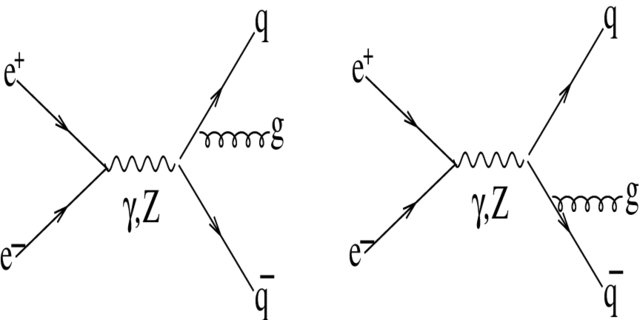
\includegraphics[width=10cm, height=3.5cm]{feynman.jpg}
       \caption*{Feynmannova diagrama za $e^+ e^- \rightarrow q \bar{q} g$.}
       \label{fig:feynman}
\end{figure}
Označimo prvega z $\mathcal{M}_1$ in drugega z $\mathcal{M}_2$ ter zapišemo prehodno amplitudo kot vsoto
\begin{equation}
       \ii \mathcal{M} = \ii \mathcal{M}_1 + \ii \mathcal{M}_2.
\end{equation}
Ob poštevanju Feynmannovih pravil:
\begin{equation}
       \begin{split}
              \frac{- \ii g^{\mu \nu}}{q^2};& \quad \text{fotonski (v Feynmanovi umeritvi tudi gluonski) propagator}, \\
              \frac{- \ii}{\slashed{p}-m} = &\frac{- \ii (\slashed{p} + m)}{p^2 - m^2}; \quad \text{fermionski propagator}, \\
              \ii e \gamma^\mu;& \quad \text{za QED vertex}, \\
              \ii g_s T_{ij}^a \gamma^\mu;& \quad \text{za QCD vertex fermion-gluon},
       \end{split}
\end{equation}
zunanjih nog ter z uvedbo $\slashed{p} \equiv \gamma^\mu p_\mu$, lahko izrazimo oba prispevka kot:
\begin{equation}
       \begin{split}
              \ii \mathcal{M}_1 = \bar{v}(k_+)( \ii e \gamma_\mu) u(k_-)\frac{-1}{q^2} \cdot 
              \bar{u_i}(p_q)(- \ii g_s T_{ij}^a) \slashed{\varepsilon}^a(p_g)
              \frac{ (\slashed{p}_q + \slashed{p}_g) }{(p_q + p_g)^2}
              (-\ii e e_q) \gamma^\mu v_j(p_{\bar{q}}), \\
              \ii \mathcal{M}_2 = \bar{v}(k_+)( \ii e \gamma_\mu) u(k_-)\frac{-1}{q^2} \cdot 
              \bar{u_i}(p_q)(-\ii e e_q)
              \frac{ (\slashed{p}_{\bar{q}} + \slashed{p}_g) }{(p_{\bar{q}} + p_g)^2}
              (- \ii g_s T_{ij}^a) \slashed{\varepsilon}^a(p_g) \gamma^\mu v_j(p_{\bar{q}}),
       \end{split}
\end{equation}
oziroma združeno
\begin{equation}
       \ii \mathcal{M} = e_q (-\ii e)^2 (-\ii g_s )\varepsilon^*_\nu (p_g)
       \bar{u}(p_q)
       \bigg[ \gamma ^\nu \frac{\ii}{\slashed{p}_q + \slashed{p}_g} \gamma^\mu - 
       \gamma^\mu \frac{\ii}{\slashed{p}_{\bar{q}} + \slashed{p}_g} \gamma_\nu \bigg]
       v(p_{\bar{q}}) \frac{-\ii}{q^2} \bar{v}(k_+) \gamma_\mu u(k_-).
\end{equation}
Za sipalni presek potrebujemo vsoto kvadratov prehodnih amplitud, povprečeno po začetnih spinih, kar lahko zapišemo kot
produkt leptonskega in kvarkovskega tenzorja:
\begin{equation}
       \overline{| \mathcal{M} |^2} = \frac{1}{4} \sum | \ii \mathcal{M}|^2 = 
       \frac{e^4 e_q^2 g_s^2}{4 s^2} L^{\mu \nu} Q_{\mu \nu},
\end{equation}
kjer je
\begin{equation}
       \begin{split}
              L^{\mu \nu} =& | \bar{v}(k_+) \gamma^\mu u(k_-) |^2 = \Tr [\slashed{k}_+ \gamma^\mu \slashed{k}_- \gamma_\nu] \\
              =& 4 [k_+^\mu k_-^\nu + k_-^\mu k_+^\nu - g^{\mu \nu}k_+ \cdot k_-], \\
              Q^{\mu \nu} =& \Big | \bar{u}(p_q) \bigg [ 
                     \frac{\slashed{\varepsilon} (p_g) (\slashed{p}_{q} + \slashed{p}_g) \gamma^\mu}{(p_{q} + p_g)^2} + 
                     \frac{\gamma^\mu (\slashed{p}_{\bar{q}} + \slashed{p}_g) \slashed{\varepsilon} (p_g)}{(p_{\bar{q}} + p_g)^2}
              \bigg ] u(p_{\bar{q}}) \Big |^2.
       \end{split}
\end{equation}
Slednjega lahko izvrednotimo s pomočjo \q{relacije} za gluone $\sum \varepsilon^\mu \varepsilon^{* \nu} \rightarrow -g^{\mu \nu}$
in spinorje $\sum u(p) \bar{u}(p) = \slashed{p} + m$ ter s preimenovanjem
\begin{equation}
       p_1 = p_q + p_g \quad \text{in} \quad p_2 = p_{\bar{q}} + p_g
\end{equation}
za voljo krajšega izraza, z upoštevanjem
$[\gamma^\mu \gamma^\nu] = 2 \gamma^\nu \gamma^\mu - 2 g_{\mu \nu}$, \hspace*{5mm}  
 ${\gamma^\mu \gamma^\nu} = - 2 g_{\mu \nu}$ ter \newline
 $ \text{Tr}(\slashed{k_1} \gamma^\mu \slashed{k_2} \gamma^\nu) = 
 4(g^{\alpha\mu} g^{\beta\nu} - g^{\alpha\beta} g^{\mu\nu} + 
 g^{\alpha\nu} g^{\mu\beta}) k_{1\alpha} k_{2\beta}$

lahko zapišemo:
\begin{equation}
       \begin{split}
              Q^{\mu \nu} =& 
              \frac{\Tr [\slashed{p}_q \gamma_\rho \slashed{p}_1 \gamma^\mu \slashed{p}_{\bar{q}} \gamma^\nu \slashed{p}_1 \gamma^\rho]}{p_1^4} +
              \frac{\Tr [\slashed{p}_q \gamma_\mu \slashed{p}_2 \gamma_\rho \slashed{p}_{\bar{q}} \gamma^\rho \slashed{p}_2 \gamma^\nu]}{p_2^4} +
              \frac{2 \Tr [\slashed{p}_q \gamma_\rho \slashed{p}_1 \gamma^\mu \slashed{p}_{\bar{q}} \gamma^\rho \slashed{p}_2 \gamma^\mu]}{p_1^2 p_2^2} \\
              =&
              \frac{16 [2(p_q p_1) (p_{\bar{q}} p_1) - p_1^2(p_q p_{\bar{q}})]}{p_1^4} +
              \frac{16 [2(p_q p_2) (p_{\bar{q}} p_2) - p_2^2(p_q p_{\bar{q}})]}{p_2^4} +
              \frac{16 [2(p_q p_1) (p_{\bar{q}} p_1) - p_1^2(p_q p_{\bar{q}})]}{p_1^2 p_2^2}.
       \end{split}
\end{equation}
Oziroma skupaj nadaljnje združeno:
\begin{equation}
       \begin{split}
              \overline{| \mathcal{M} |^2} =&  
              \frac{E^2 g^2 e^4}{4 s^2} (-g_{\nu \sigma})
              \Tr [\gamma_\mu \slashed{k}_+ \gamma_\rho \slashed{k}_-] \\
              & \quad \quad \Tr
              \bigg[ \bigg( \gamma ^\nu \frac{\ii}{\slashed{p}_q -
              \slashed{p}_g} \gamma^\mu - \gamma^\mu \frac{\ii}{\slashed{p}_{\bar{q}} + \slashed{p}_g} \gamma ^\nu \bigg)
              \slashed{p}_{\bar{q}}
              \bigg( \gamma ^\rho \frac{\ii}{\slashed{p}_q - \slashed{p}_g} \gamma^\sigma - 
              \gamma^\sigma \frac{\ii}{\slashed{p}_{\bar{q}} + \slashed{p}_g} \gamma ^\rho \bigg)
              \slashed{p}_q \bigg]
              \\
              =& \frac{4 E^2 g^2 e^4}{3s^2} (8p_q \cdot p_{\bar{q}})
              \bigg [
              \frac{4(p_q \cdot p_{\bar{q}})(p_q \cdot p_{\bar{q}} + q\cdot p_g)}{(p_q + p_g)^2(p_{\bar{q}}+p_g)^2}
              +
              \Big(
                     \frac{1}{(p_q + p_g)^4} + \frac{1}{(p_{\bar{q}} + p_g)^4}
              \Big)
              \big (2 (p_q \cdot p_g)(p_{\bar{q}} \cdot p_g) - \mu^2 (p_q \cdot p_{\bar{q}}) \big)
              \bigg].
       \end{split}
\end{equation}

Upoštevamo še (\ref*{eq:pokazi}) za \underline{brezmasne delce}, od koder direktno sledi:
\begin{equation}
       p_i \cdot p_j = \frac{s (1 - x_k)}{2}.
\end{equation}
Prehodno amplitudo za naš proces lahko tedaj izrazimo kot
\begin{equation}
       \begin{split}
       \overline{| \mathcal{M} |^2} =& \frac{8 e^4 e_q^2 g_s^2}{s^2} 
       \bigg [
              \frac{1-x_2}{1-x_1} + \frac{1-x_1}{1-x_2} + \Big (\frac{2}{(1-x_1)(1-x_2)} - \frac{2}{1-x_1} - \frac{2}{1-x_2} \Big)
       \bigg] \\
       =& \frac{8 e^4 e_q^2 g_s^2}{3 s} \frac{x_1^2 + x_2^2}{(1-x_1)(1-x_2)}
       \end{split}
\end{equation}








\subsection{Sipalni presek}
S tem rezultatom lahko zdaj zapišemo sipalni presek v težiščnem sistemu.
Upoštevamo, da je vpadni tok v težiščnem sistemu $|v_{e+} - v_{e-}| = 2$ in $2E_{e+} = 2E_{e-} = \sqrt{s}$,
v faznem integralu $\mu \rightarrow 0$
\begin{equation}
       \begin{split}
              \frac{\dd \sigma}{\dd x_1 \dd x_2} =& \frac{1}{2E_{p_1}2E_{p_2} |v_{p_1} - v_{p_2}|}
              \frac{1}{128 \pi^3} \Big ( \frac{1}{4}\sum | \mathcal{M}|^2 \Big)
              \\
              =& \frac{4 \pi \alpha^2}{3s} \cdot 3 e_q^2 \cdot \frac{\alpha_g}{2 \pi}
              \frac{x_1^2 + x_2^2}{(1-x_1)(1-x_2)},
       \end{split}
\end{equation}
Izraz ima divergence pri $x_1 =1$ in $x_2 =1$.
Vzemimo primer, ko gre $x_1 \rightarrow 1$.
Iz (\ref*{eq:pokazi}) tedaj sledi:
\begin{equation}
       s(1-x_1) = 2 p_{\bar{q}} p_g = 2 E_{\bar{q}} E_g (1-\cos \theta_{\bar{q} g}).
\end{equation}
Vidimo, da če se kateri od $x_i$ približa vrednosti 1, gre kot med izsevanim gluonom in kvarkom proti nič.
Za tri hadronske curke je torej relevantno osrednje območje na sliki \ref{fig:meje}.

Če ponovno izvrednotimo povprečje kvadratnih amplitud z neničelno maso $\mu$,
dobimo
\begin{equation}
       \overline{ | \mathcal{M} |^2} = \frac{8 e_q^2 g^2 e^4}{3s} F(x_1, x_2, \mu^2/s),
\end{equation}
kjer je
\begin{equation}
       F(x_1, x_2, \mu^2/s) = \frac{2(x_1 + x_2 -1 + \frac{\mu^2}{s})(1+ \frac{\mu^2}{s})}
       {(1-x_1)(1-x_2)}
       + 
       \bigg[ \frac{1}{(1-x_1)^2} + \frac{1}{(1-x_2)^2}  \bigg ]
       \Big( (1-x_1)(1-x_2) - \frac{\mu^2}{s} \Big).
\end{equation}
Pripadajoč sipalni presek pa je potem
\begin{equation}
       \begin{split}
              \sigma(e^+ e^-  \rightarrow q \bar{q} g) =&
              \frac{1}{2E_{p_1} 2E_{p_2} |v_{p_1}- v_{p_2}|} \frac{s}{128 \pi^3} \int \dd x_1 \dd x_2
              \Big ( \frac{1}{4} \sum |\mathcal{M}|^2 \Big)
              \\ =&
              \frac{4 \pi \alpha^2}{3s} \cdot 3 e_q^2 \cdot \frac{\alpha_s}{2 \pi}
              \int_0^{1-\mu^2/s} \dd x_1 \int_{1-x_1 - \mu^2/s}^{1-\frac{t}{s(1-x_1)}} \dd x_2
              F(x_1, x_2, \mu^2/s)
              \\ =&
              \frac{4 \pi \alpha^2}{3s} \cdot 3 e_q^2 \cdot \frac{\alpha_s}{2 \pi}
              \Big[ \ln^2\frac{\mu^2}{s} + 3 \ln \frac{\mu^2}{s} + 5 - \frac{1}{3 \pi^2} + \mathcal{O}(\mu^2) \Big].
       \end{split}
\end{equation}


%Če se vrnemo na začetek in izvedemo integracijo po Feynmannovih parametrih
%\begin{equation}
%       F_1(q^2 = s) = E^2 - \frac{E^2 \alpha_g}{4 \pi}
%       \bigg [
%       \ln^2 \frac{\mu^2}{s} + 3 \ln \frac{\mu^2}{s} + \frac{7}{2} - \frac{1}{3} \pi^2
%       - \ii \pi \big (2 \ln \frac{\mu^2}{s} + 7 \big ) + \mathcal{O}(\mu^2)
%       \bigg]
%\end{equation}
%Od koder dobimo spremembo v sipalnem preseku, ki je potem oblike
%\begin{equation}
%       \sigma(e^+ e^-  \rightarrow q \bar{q}) =
%       \frac{4 \pi \alpha^2}{3s} \cdot 3 E^2
%       \bigg [1 - \frac{\alpha_s}{2 \pi}
%              \Big[ \ln^2\frac{\mu^2}{s} + 3 \ln \frac{\mu^2}{s} + 5 - \frac{1}{3 \pi^2} + \mathcal{O}(\mu^2) \Big]
%       \bigg ].
%\end{equation}


\section{Zaključek}
Če v upoštev vzamemo še najnižji popravek gluona h kvarkovskemu verteksu, se v limiti $\mu \rightarrow 0$
divergence ravno pokrajšajo.
Navedimo samo končni rezultat:
\begin{equation}
       \sigma(e^+ e^-  \rightarrow q \bar{q} + q \bar{q} g) =
       \frac{4 \pi \alpha^2}{3s} \cdot 3 e_q^2
       \bigg [1 - \frac{3 \alpha_g}{4 \pi} \bigg ].
\end{equation}

Hadronizacija iz H.M. ...




\vspace{1cm}
\printbibliography

\end{document}